\section{Post-processing and drawing} \label{sec:ideal_exp_net2g}
%------------------------------------------------------
In this section, we explain post-processing and the method of drawing the calculation result.  In the tutorial, the distributed files in \netcdf format are merged into one file and converted into simple binary form ({\grads} form) that can be directly accessed. The binary form makes it easy for users to analyze the result. Link to the post-processing tool \verb|net2g| compiled  in Section \ref{sec:source_net2g}:
\begin{verbatim}
  $ ln -s ../../../util/netcdf2grads_h/net2g  ./
\end{verbatim}

The method of execution of \verb|net2g| is the same as that of \scalerm, i.e.,
\begin{verbatim}
 $ mpirun -n [the number of the processes] ./net2g [the configuration file]
\end{verbatim}
The configuration file \verb|sample/net2g_R20kmDX500m.conf| is intended for special uses of \verb|net2g|.
Give this configuration file to \verb|net2g| and execute it as follows:
\begin{verbatim}
  $ cp  sample/net2g_R20kmDX500m.conf  ./net2g_R20kmDX500m.conf
  $ mpirun  -n  2  ./net2g  ./net2g_R20kmDX500m.conf
\end{verbatim}
If there is no error message and the following message is displayed to the standard output,
the conversion is completed without problem:
\msgbox{
\verb|+++ MPI COMM: Corrective Finalize| \\
}

The execution of net2g should be handled,
so that the number of MPI processes is identical to, or a divisor of, that used for the run of \scalerm. The following six files are generated under the same directory by this execution:
\begin{alltt}
  QHYD_d01z-3d.ctl
  QHYD_d01z-3d.grd
  V_d01z-3d.ctl
  V_d01z-3d.grd
  W_d01z-3d.ctl
  W_d01z-3d.grd
\end{alltt}
The ``grd'' files are the converted files in the simple binary form of direct access
({\grads} form) obtained by merging the divided files,
whereas the ``ctl'' files are used to render them readable by \grads.
%In this case, these files contain U (horizontally eastern wind), W (vertical wind), and QHYD (mass concentration of total hydrometeors).

To confirm whether the calculation is satisfactory,
draw a figure using \grads script \verb|checkfig_ideal.gs|.
Note that the grammar depends on the version of \grads.
If a warning appears, the \grads script should be rewritten appropriately:
\begin{verbatim}
  $ grads -blc checkfig_ideal.gs
\end{verbatim}
If it is successfully completed, the following files are generated:

\begin{verbatim}
   ideal_QHYD.png
   ideal_W.png
\end{verbatim}
The same figures as Fig. \ref{fig_ideal} can be found in the simulation,
and post-processing is successfully concluded.

\begin{figure}[htb]
\begin{center}
  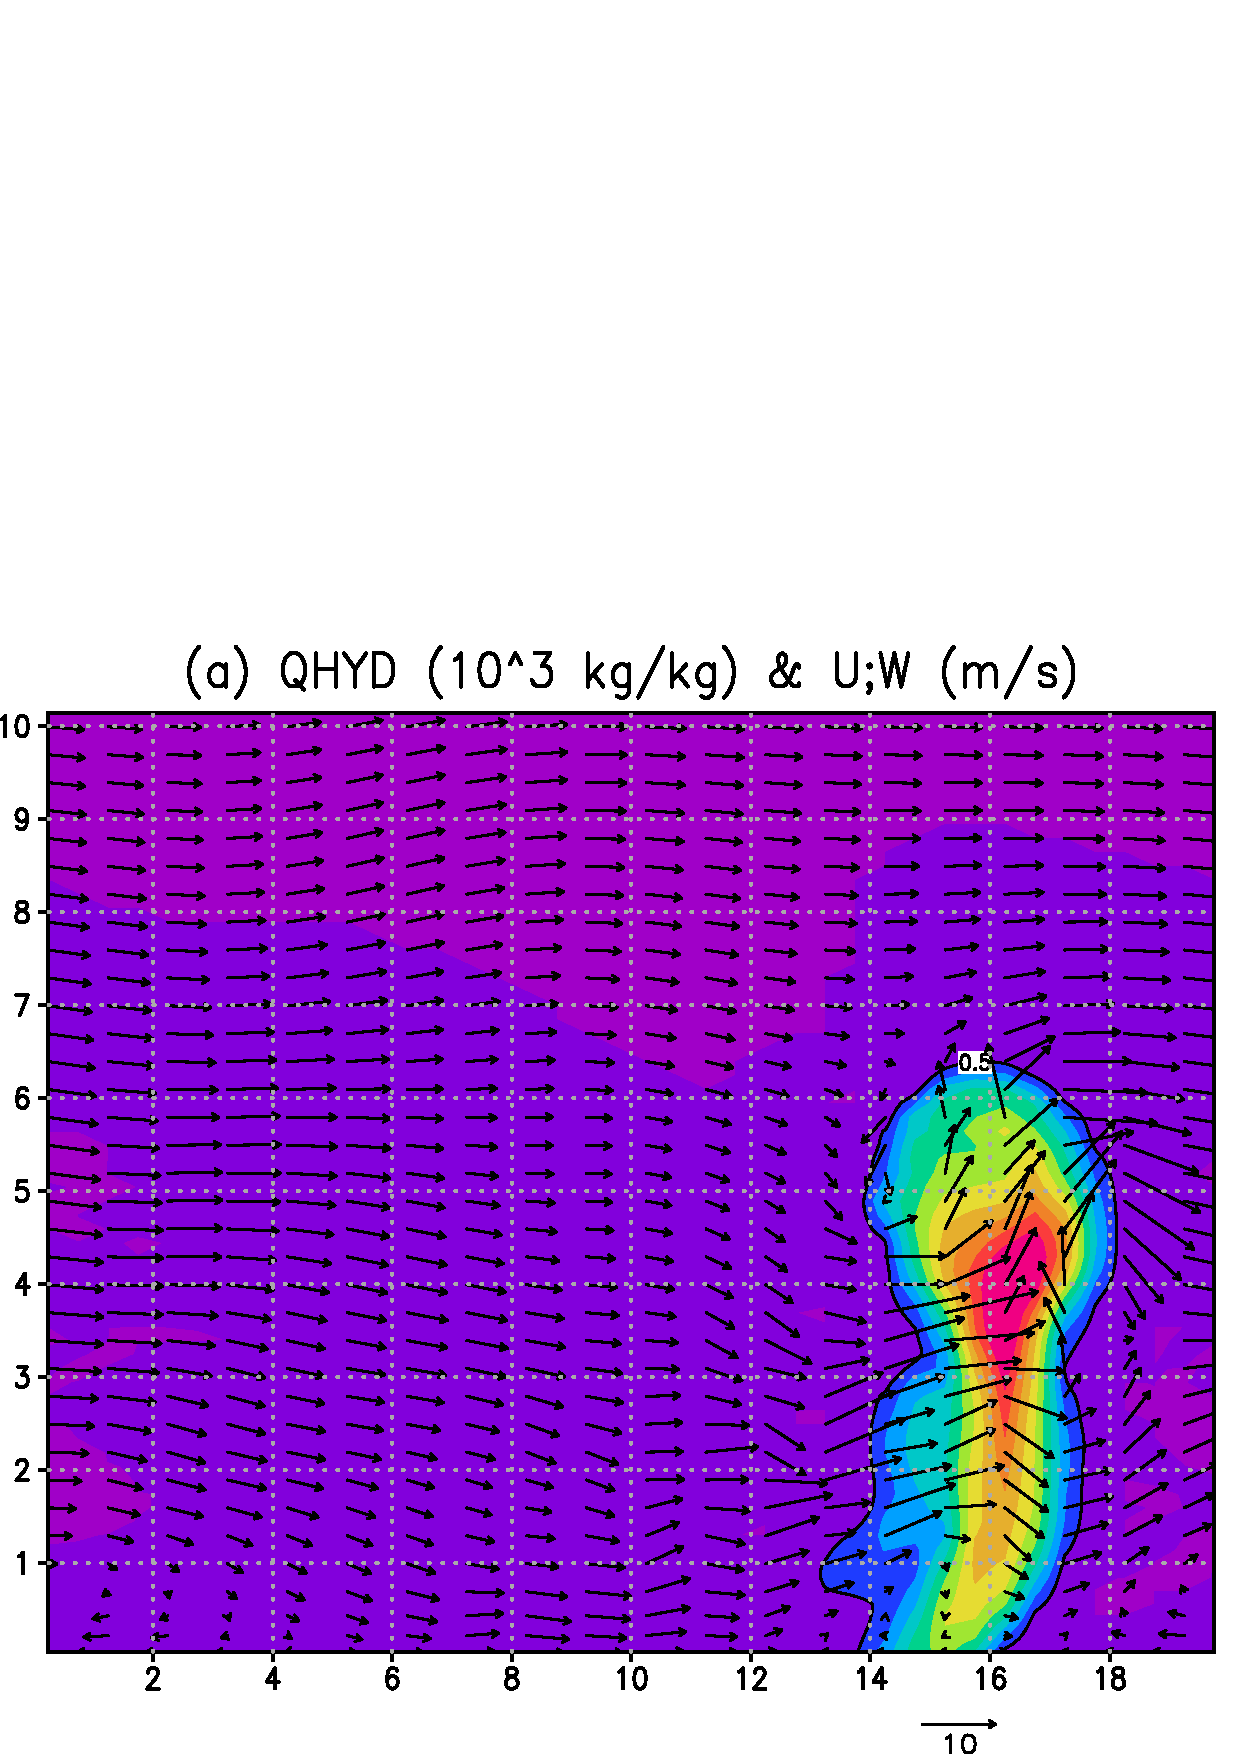
\includegraphics[width=0.65\hsize]{./figure/ideal_qhyd.pdf}\\
  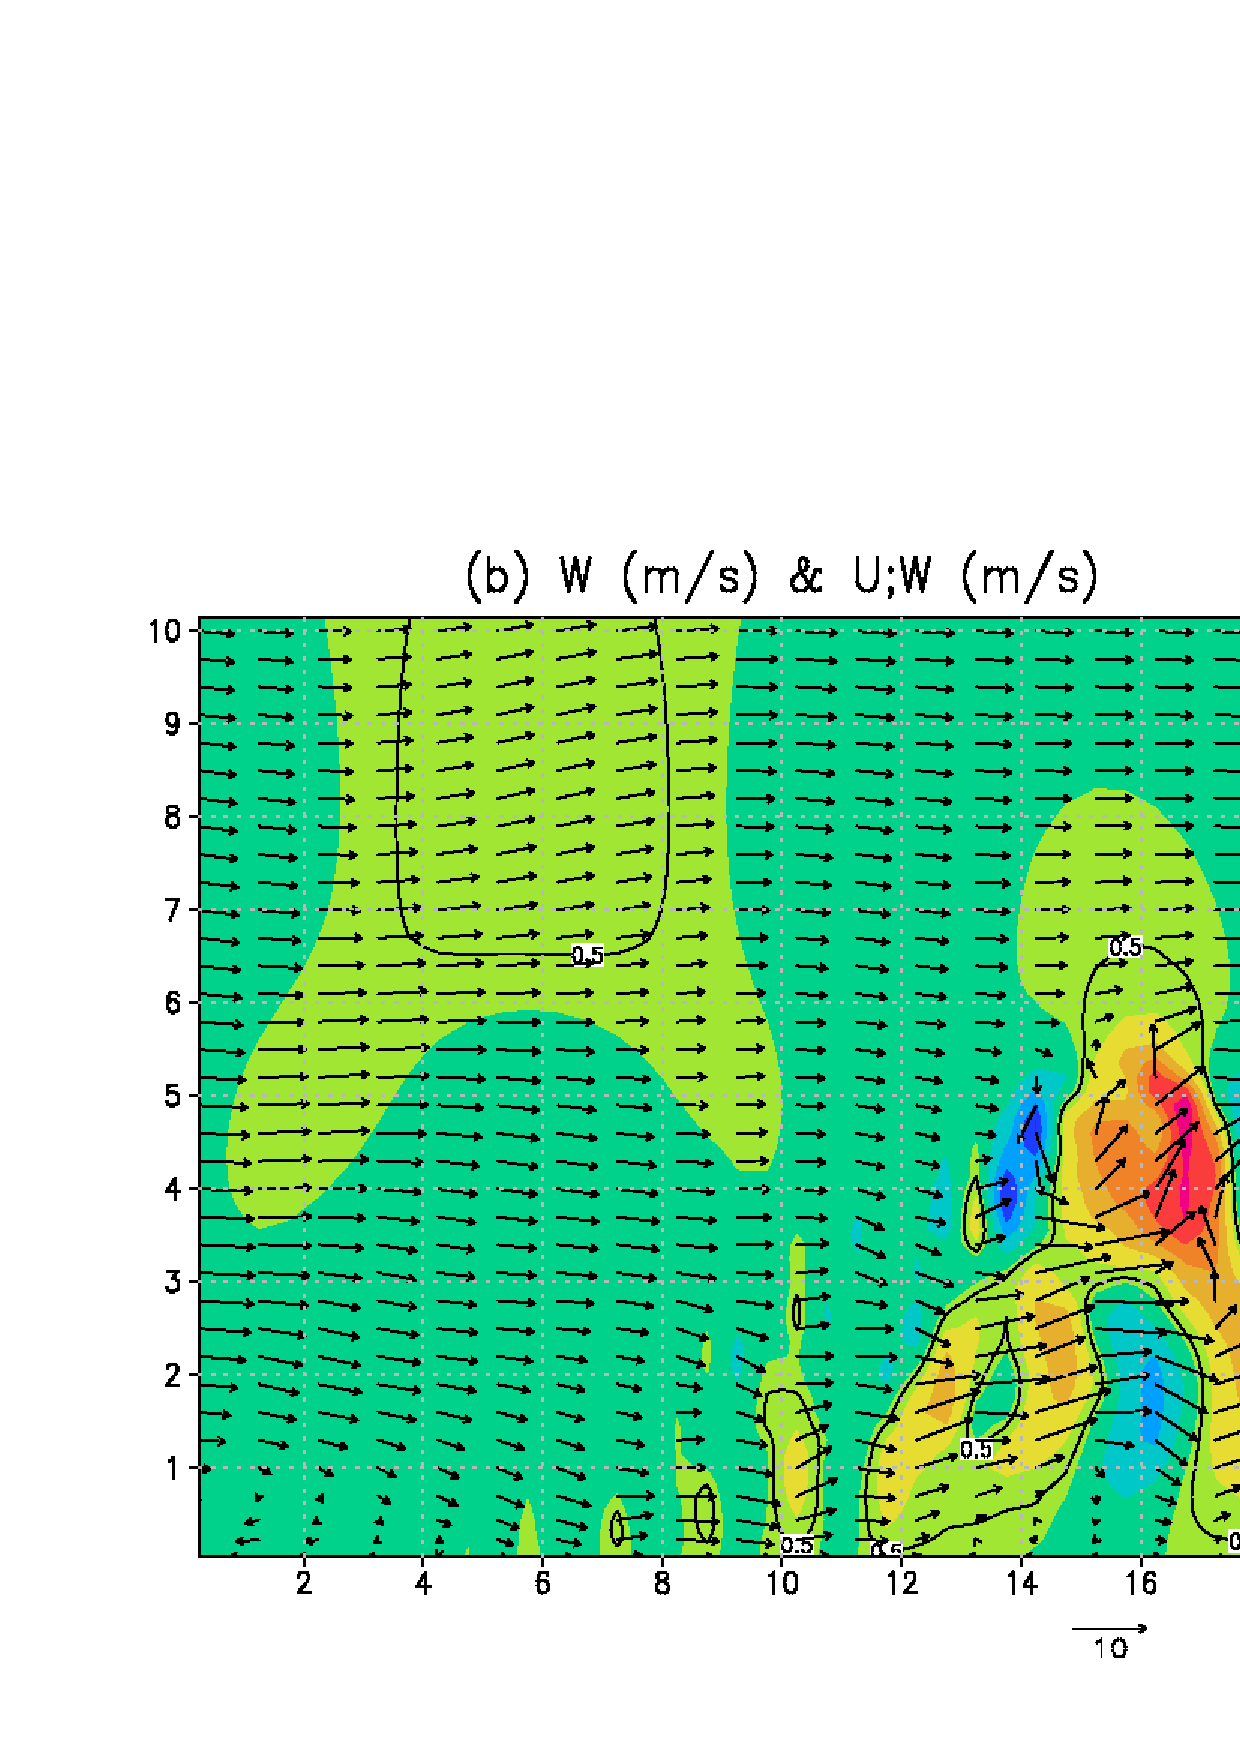
\includegraphics[width=0.65\hsize]{./figure/ideal_W.pdf}\\
  \caption{The horizontal-vertical cross-section after t=1200 s (20 minutes later);
            Figure (a) shows the mass concentration of the hydrometeor, and 
            Figure (b) shows the vertical velocity. 
            In both of figures, the vector indicates flow.}
  \label{fig_ideal}
\end{center}
\end{figure}

To convert the result of the output into binary data for other variables,
add them to \nmitem{VNAME} in \namelist{VARI} in the configuration file \verb|net2g_R20kmDX500m.conf|:
\editbox{
\verb|&VARI|\\
\verb| VNAME       = "V","W","QHYD"|\\
\verb|/|\\
}
To check the output variable in the history file, use \verb|ncdump| of {\netcdf}.
Refer to Section \ref{sec:net2g} for the detailed use of net2g.

